\documentclass{article}
\usepackage{graphicx}
\usepackage{float}
\title{Technical Skill Enchancer(TeaSk)}
\author{Daniel Creanga si Narcis Zaharia}
\date{April 19, 2019}

\begin{document}

\maketitle
\bigskip
\tableofcontents
\break


\section{Introducere}
Proiectul reprezinta o aplicatie web care permita utilizatorului sa fie la curent cu cele mai noi evenimente(conferinte, stagii, etc.). 

Utilizatorii isi vor putea urmarii progresul pe care il fac in anumite limbaje de programare prin asistarea la aceste evenimente si prin anumite actiuni pe care le fac pe GitHub, daca aleg sa isi foloseasca acel cont in aplicatie.

Stagiile si conferintele vor fi preluate de pe siteuri dar vor si putea fi adaugate de administrator. Recomandarile vor fi facute in functie de interesul de pe GitHub.

Odata ce utilizatorul gaseste stagiul sau conferinta dorita acesta poate accesa o pagina in care se gasesc toate detaliile, mai apoi acesta poate accesa pagina companiei si apoi lua legatura cu ei. 

\bigskip

\section{Use Cases}

Utilizatorul se poate inregistra in aplicatie cu un username unic, un email unic, o parola, un nume si un prenume. Fara cont, utilizatorii nu pot naviga pe pagina principala pe care vor fi afisate. Dupa inregistrare un utilizator isi va putea adauga contul de GitHub in aplicatie, care cu ajutorul API-ului de la GitHub ne va oferi informatii despre nivelul acestuia la anumite limbaje de programare.
Utilizatorul isi poate vedea statisticile personale pe baza skillurilor acestuia. Skillul reprezinta nivelul utilizatorului la un anumit limbaj de programare si este reprezantat de un numar intre 1 si 10.
Skillul va fi calculcat pe baza activitatii recente a utilizatorului pe GitHub daca are contul conectat. Evenimentele la care un utilizator participa ii pot creste nivelul skillului daca acestea au un nivel apropiat de cel al utilizatorului. Astfel daca un utilizator participa la un eveniment al carui nivel difera prin cel mult un punct de cel al utilizatorului, atunci nivelul utilizatorului va creste cu 0.25.
Pe baza acestor skilluri, utilizatorul va putea filtra evenimentele astfel incat sa apara doar cele prin care, nivelul utilizatorului poate creste.

Daca utilizatorul are acces administrativ, acesta va putea adauga, modifica sau sterge evenimente.

Utlilzatorul va putea accesa pagina de setari unde va putea sa isi schimbe parola dar si emailul, cu un alt email care nu exista deja in baza de date.


\begin{figure}[H]
	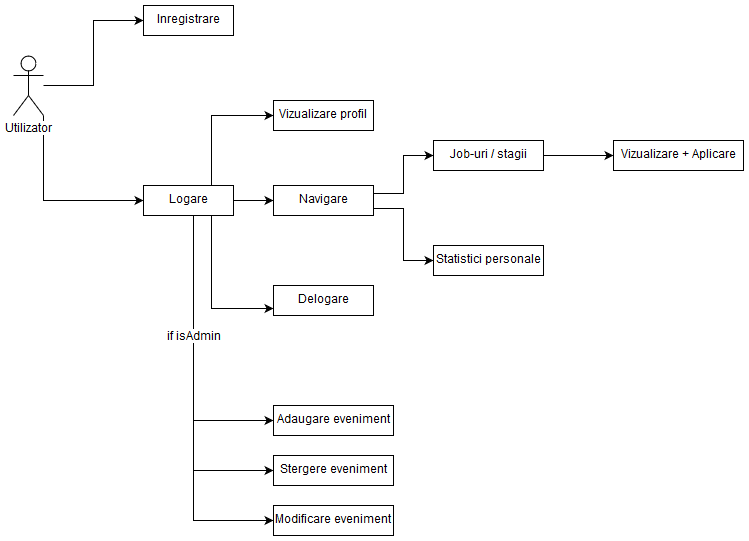
\includegraphics[width=1\textwidth]{Use-Case-Diagram.png}
	\caption{Use Case Diagram}
\end{figure}

\bigskip

\section{Arhitectura aplicatiei}

Aplicatia va fi scrisa in PHP si JavaScript si va folosi o baza de date MySQL. Aplicatia va fi folosi API-ul de la GitHub pentru a putea sa-i dea un nivel unui user la un anumit limbaj de programare. 

Astfel aplicatia va avea cate un view, ce consista din html si css pentru fiecare pagina web. Controllerele vor fi raspunde la requesturile facute de paginile web, iar acestea vor folosi datele din Models. 

Modelele sunt reprezentate prin clasele folosite in aplicatie (Users, Events, Skills, etc.).


\subsection{Arhitectura MVC}

\begin{figure}[H]
	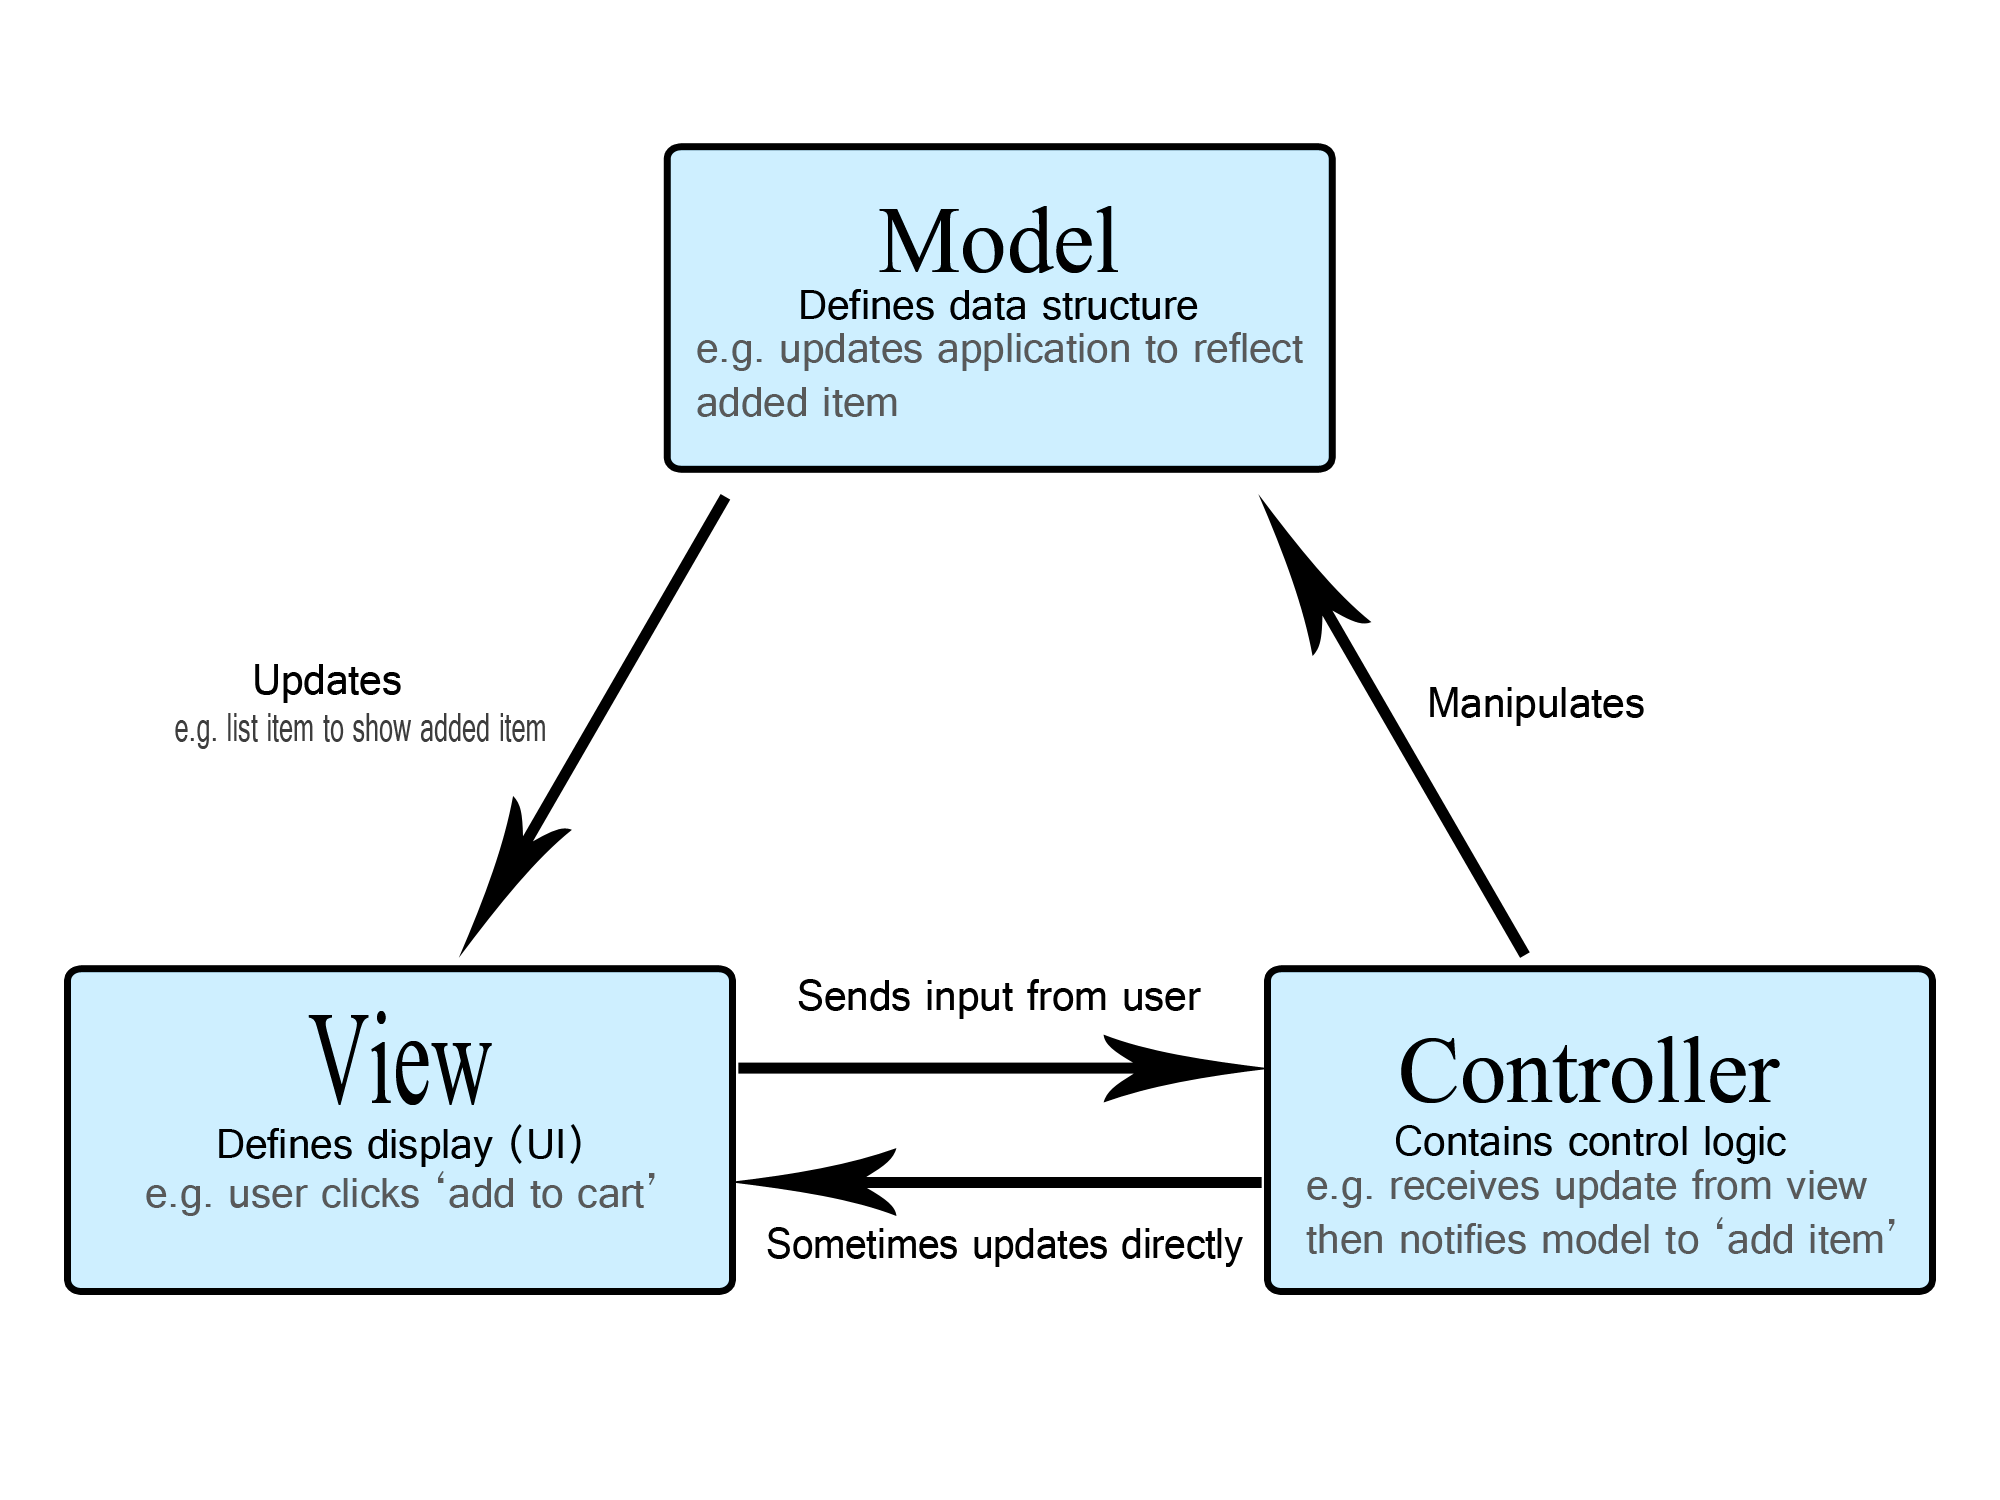
\includegraphics[width=1\textwidth]{mvc.png}
	\caption{Model View Controller diagram}
\end{figure}
\bigskip

Aplicatia va folosi o arhitectura de tip Models, Views, Controllers, astfel aplicatia va fi cumpusa dintr-un set de modele, controallere si viewuri.

Modelul reprezinta datele si regulile care se aplica acestor date, care reprezinta concepte pe care aplicatia le administreaza. Astfel, arhitectura va contine cate un model pentru utilizatori, evenimente, skilluri si internshipuri. Intre reprezentarea acestor modele in baza de date si reprezentarea lor in aplicatie va exista un layer intermediar pentru ruperea logicii legate de baza de date si securizarea datelor. 

\begin{figure}[H]
	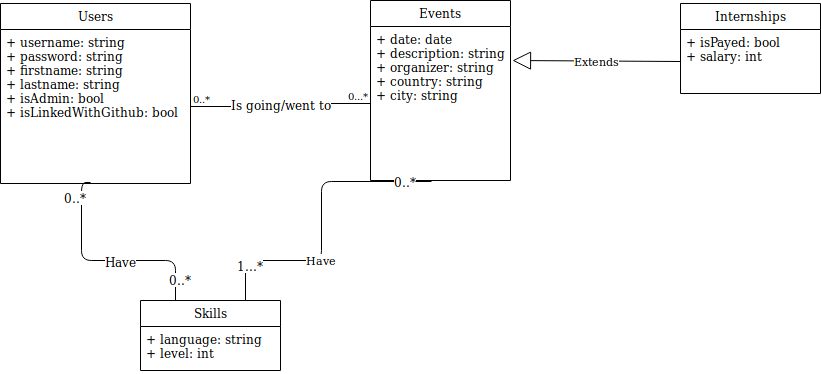
\includegraphics[width=1\textwidth]{Class-Diagram.png}
	\caption{Diagrama claselor folosite}
\end{figure}
\bigskip

Aceste modele vor fi folosite si in baza de date, pastrandu-se si un istoric al evenimentelor la care un utilizator a fost si un alt istoric pentru fiecare evolutie a unui utilizator la un anumit skill, pe baza carora se vor afisa statistici.

Viewurile ofera moduri diferite de prezentare a datelor primite de la model. Acestea sunt sabloane in care datele sunt completate. Va exista cate un view diferit pentru fiecare pagina din aplicatie (login/register, newsfeed, setari si statistici).

Controllerul gestioneaza solicitarile utilizatorilor (primite ca cereri HTTP GET sau POST cand utilizatorul interactioneaza cu un view). Controllerul va apela si coordona resursele si obiectele necesare pentru a efectua actiuniile utilizatorulilor. Controllerul va apela modelul adecvat pentru sarcina si apoi va selecta viewurile corespunzatoare.

\end{document}
